\chapter{The GLLAMM for dichotomous outcomes} \label{chap:framework}

The Generalized Linear Latent and Mixed Model (GLLAMM) is a framework that unifies a wide range of latent variable models. Developed by Rabe-Hesketh, Skrondal and colleagues \cite{Rabe_et_al_2004a, Rabe_et_al_2004b, Rabe_et_al_2004c, Skrondal_et_al_2004a, Rabe_et_al_2012}, the method was motivated by the need of a Multilevel Structural Equation Model (MSEM) that accommodates for unbalanced data, noncontinuous responses and the use of cross-level effects among latent variables. The authors focused its development mainly from the frequentist perspective, however, they offered a general guidance on implementing the models under the bayesian framework (see \citet{Skrondal_et_al_2004a}).


\section{Model motivation} \label{sect:motivation}

Consider a large standardized assessment composed of three sub-test designed to evaluate the reading comprehension, mathematical reasoning, and pedagogical knowledge of teachers; where each sub-test is composed of several dichotomously scored items. 

Focusing now on the first sub-test, the items were designed to measure three hierarchically nested sub-dimensions of reading comprehension: literal, inferential, and reflective abilities. Therefore, the items ``point-out" only to one of the aforementioned scales. Furthermore, its is assumed the three sub-dimensions are all that is needed to measure the reading comprehension ability, effectively making this scale the highest level latent variable in the model, similar to a hierarchical Confirmatory Factor Analysis (CFA). Finally, the items are bundled in groups of five to a common text or passage, i.e. testlets, that provides the stimulus over which the individual will be assessed. Figure \ref{fig:design} shows the path diagram of the hypothesized dimensional structure, for the hierarchical cross-classified IRT model corresponding with the aforementioned instrument design.

\begin{figure}[h] \label{fig:design}
	\centering
	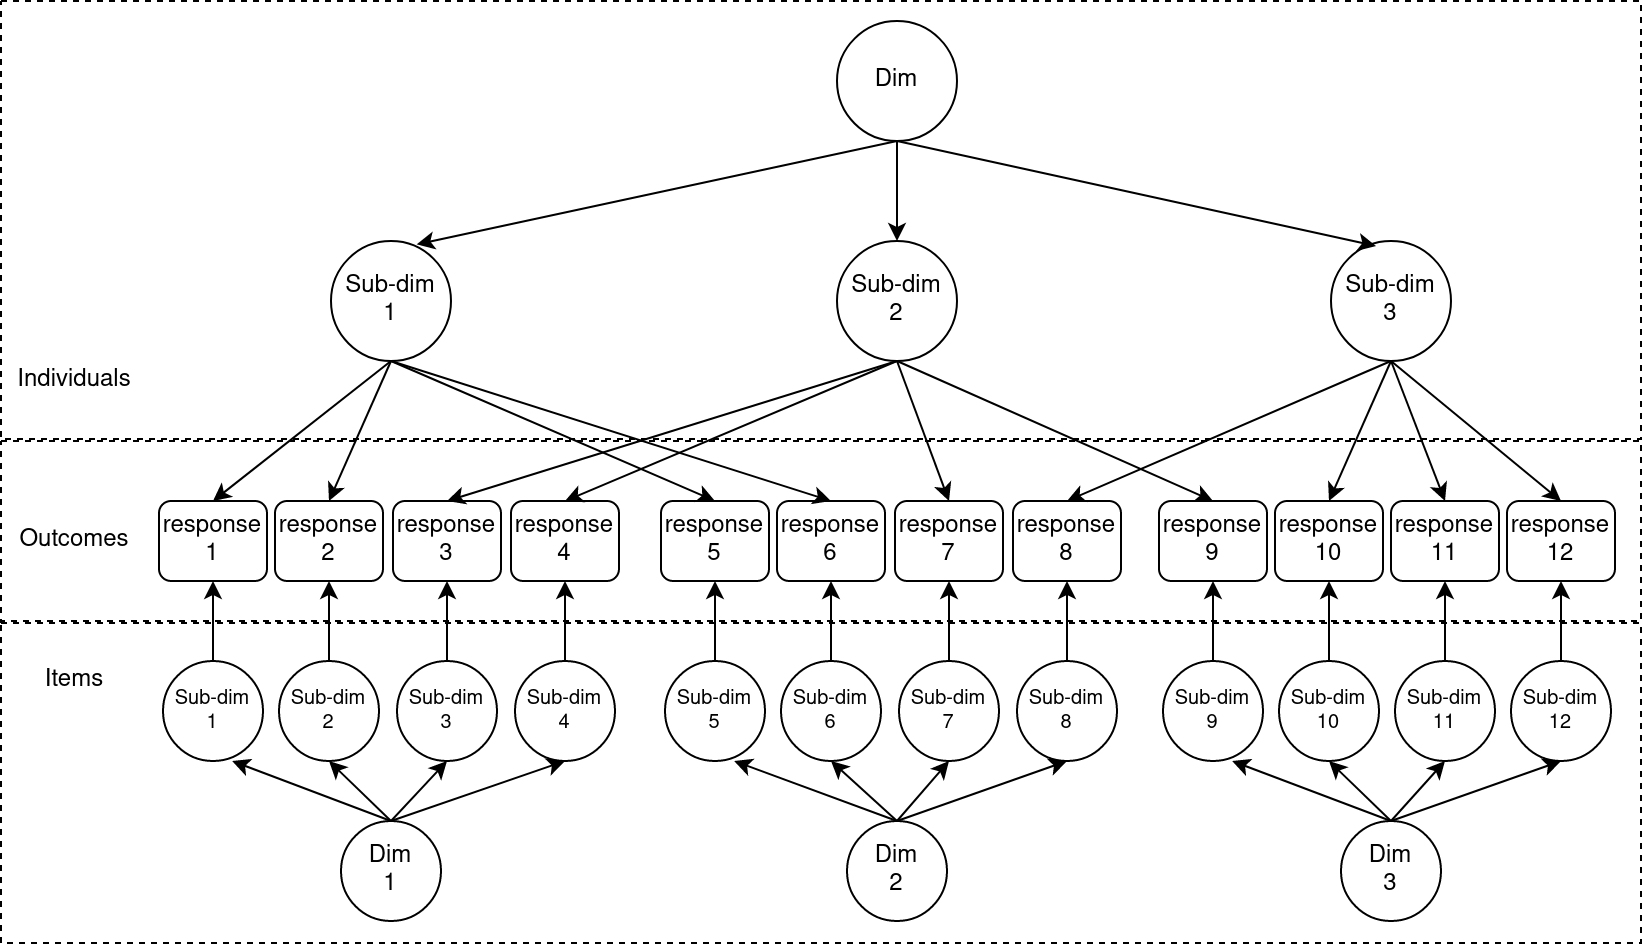
\includegraphics[width=0.85\textwidth]{instrument_design.png}
	\caption{Path diagram of the dimensional structure for a hierarchical cross-classified IRT model. Squares represent dichotomous manifest variables, and circles represent latent variables. The figure is based on reduced set of items, while errors and scales of the latent variables are not represented. Different sub-dimensions in the individuals block represent the literal, inferential and reflective abilities, while in the items blocks represent the items' difficulties. The dimensions in the individuals block represent the reading comprehension ability, while in the items block represent the multiple testlets.}
\end{figure}

With the purpose of providing an easier motivation of the model, we will not consider yet the cluster effects; however, later in the presentation we will show how easy is to introduce them in the model. Just for future reference, under this example, one expects to observe clustering effects because individuals from different regions did not have the same educational opportunities, effectively causing differences among individuals at a regional level.


\section{Model definition} \label{sect:definition}

Following \citet{Rabe_et_al_2004a, Rabe_et_al_2004b}, we continue defining the GLLAMM in two parts: (i) the response model, and (ii) the latent structure. Furthermore, conditional on the latent variables, the response model is defined by a Generalized Linear Model (GLM) \cite{Nelder_et_al_1972, Nelder_et_al_1989} with a systematic part, and a distributional part. The latter composed of a linear predictor and a link function.

If the reader is interested in cases where the outcome is not dichotomous, refer to Appendix \ref{appA1:links}.

\subsection{Response model} \label{s_sect:response}

In the distributional part, the dichotomous items $y_{jkd}$ are modeled at the first level by a Bernoulli probability mass function $f(\cdot)$, in the following form:
\begin{equation} \label{eq:distributional}
	\begin{split}
		f \left( y_{jkd}=1 \; | \; \pmb{\beta}, \pmb{\lambda}, \pmb{\eta}, \mathbf{X}, \mathbf{Z} \right) &= p_{jkd}^{n} (1 - p_{jkd})^{1-n}
	\end{split}
\end{equation}

\noindent where $n$ denotes if the item was endorsed or not in the Bernoulli trial. On the other hand, in the systematic part, the probability of endorsing the item $p_{jkd}$ is linked to a linear predictor $v_{jkd}$ through an inverse-link function $h(\cdot)$, in the following form:
\begin{equation} \label{eq:systematic}
	\begin{split}
		P\left[ y_{jkd}=1 \; | \; \pmb{\beta}, \pmb{\lambda}, \pmb{\eta}, \mathbf{X}, \mathbf{Z} \right] &= p_{jkd} = h(v_{jkd})
	\end{split}	
\end{equation}

\noindent where the inverse-link function can be defined in three ways:	
\begin{equation} \label{eq:response_dich1}
	h(x) = 
	\begin{cases}
		exp(x)[1 + exp(x)]^{-1} \\
		\Phi(x)  \\
		exp(-exp(x))
	\end{cases}
\end{equation}

\noindent corresponding to the logistic, standard normal $\Phi(x)$ (with no closed form), and Gumbel (extreme value type I) cumulative distributions, respectively. In terms of link functions $g(\cdot) = h^{-1}(\cdot)$, the distributions corresponds to the well known logit, probit and complementary log-log link functions, respectively. Finally, the linear predictor is defined by:
\begin{equation} \label{eq:linear_predictor}
	v_{jkd} = \mathbf{X}_{j} \pmb{\beta} + \sum_{m=2}^{M} \sum_{k=1}^{K_{(m)}} \eta_{k}^{(m)} \mathbf{Z}_{k}^{(m)} \pmb{\lambda}_{k}^{(m)} + \sum_{l=2}^{L} \sum_{d=1}^{D_{(l)}} \eta_{d}^{(l)} \mathbf{Z}_{d}^{(l)} \pmb{\lambda}_{d}^{(l)}
\end{equation}

\noindent where individuals are indexed by $j = 1, \dots, J$, and $J$ represents the total number of individuals in the sample. Item are indexed with $k= 1, \dots, K_{(m)}$, where $K_{(m)}$ represents the number of dimensions at level $m=2,\dots, M+1$, and $M$ represent the number of levels in the items block. Finally, individuals' dimensions are indexed by $d=1, \dots, D_{(l)}$, where $D_{(l)}$ represents the number of dimensions at level $l=2, \dots, L+1$, and $L$ denotes the number of levels observed in the individuals block. Using figure \ref{fig:design} as a reference, we would have $M=2$ levels in the items bock, where $K_{2}=12$ corresponding to the items difficulties, and $K_{3}=3$ corresponding to the testlets. Similarly, we would have $L=2$ levels in the individuals block, with $D_{2}=3$ corresponding to the literal, inferential and reflective abilities, and $D_{3}=1$ corresponding to the reading comprehension latent variable. 

On the other hand, $\mathbf{X}_{j}$ represents  the design matrix of additional explanatory variables, that maps the parameter vector $\pmb{\beta}$ to the linear predictor, where $\mathbf{X} = \left[ \mathbf{X}_{1}^{T}, \dots, \mathbf{X}_{J}^{T} \right]^{T}$ is the  ``stacked" representation for all individuals. Similarly $\eta_{m}^{(l)}$ the $m$th latent variable at level $l$ ($m=1, \dots, M_{(l)}$ and $l=1, \dots, L$), and $\mathbf{Z}_{m}^{(l)}$ a design matrix that maps the vector of loadings $\pmb{\lambda}_{m}^{(l)}$ to the $m$th latent variable at level $l$ with $\pmb{\eta}=\left[\eta^{(2)T}, \dots, \eta^{(L)T}\right]^{T}$ and $\mathbf{Z}=\left[\mathbf{Z}^{(2)T}, \dots, \mathbf{Z}^{(L)T}\right]^{T}$, as the "stacked" vector of latent variables, and the "stacked" design matrices of explanatory variables, for all $L$ levels, respectively. Additionally, $\pmb{\eta}^{(l)}=\left[\eta_{1}^{(l)}, \dots, \eta_{M_{(l)}}^{(l)}\right]^{T}$ and $\mathbf{Z}^{(l)}=\left[\mathbf{Z}_{1}^{(l)T}, \dots, \mathbf{Z}_{M_{(l)}}^{(l)T}\right]^{T}$, denotes the vector of latent variables, and the "stacked" design matrix of explanatory variables, at level $l$, respectively.



The model departs from the traditional multivariate framework for formulating factor and structural models, i.e. a wide data format\footnote{ The subject’s repeated outcomes are stored in a single row, with multiple response vectors. Moreover, different variables are appended column-wise to the outcome data. }, and adopts a univariate approach, i.e. a long data format\footnote{ The subject’s repeated outcomes are stored in a single ``stacked" response vector with as many rows as there are repeated measurements. Moreover, different variables are appended column-wise to the outcome data, distinguished from each other, by a design matrix. }. 





\subsubsection{Cluster effect} \label{ss_sect:clusters}

Much like the Generalized Linear Mixed Model framework (GLMM), the GLLAMM allows to model heteroscedasticity, and over- or under-dispersion by adding random effects to the linear predictor, at level $1$. The types of responses, in which such characteristics can be modeled, are the following:
	
In a more straightforward way, we model over- or under-dispersion by modifying equation (\ref{eq:link_dich}), to include random intercepts at level $1$, in the following form:
\begin{equation} \label{eq:link_dich1}
	\begin{split}
		\mu &= P[y=1 | \mathbf{X}, \mathbf{Z}, \pmb{\eta}] \\
		&= \pi \\
		&= h(\kappa - v + \pmb{\alpha}^{T}\mathbf{Z^{(1)}})
	\end{split}	
\end{equation}
	
	


\subsection{Latent structure} \label{s_sect:struct}
The structural model for the latent variables has the form:
\begin{equation} \label{eq:structural_model}
	\def\sss{\scriptstyle}
	\setstackgap{L}{12pt}
	\def\stacktype{L}
	\pmb{\eta} = \stackunder{\mathbf{B}}{\sss (M \times M)} \stackunder{\pmb{\eta}}{\sss (M \times 1)} + \stackunder{\pmb{\Gamma}}{\sss (M \times Q)} \stackunder{\mathbf{W}}{\sss (Q \times 1)} + \stackunder{\pmb{\zeta}}{\sss (M \times 1)}
\end{equation}
where $\mathbf{B}$ and $\pmb{\Gamma}$ are parameter matrices that maps the relationship between the latent variables $\pmb{\eta}$, and the vector of "stacked" covariates $\mathbf{W}$, respectively; $\pmb{\zeta}$ is a vector of errors or disturbances, and $M = \sum_{l} M_{l}$. Notice that while equation (\ref{eq:structural_model}) resembles to single-level structural equation models, the main difference lies in the fact that the latent variables may vary at different levels. Additionally, considering that $\pmb{\eta}$ has no feedback effects, and it is permuted and sorted according to the levels, $\mathbf{B}$ is defined as a strictly upper triangular matrix. In this regard, it is important to mention that,
\begin{enumerate}
	\item The absence of feedback loops implies that the method deals with non-recursive models, i.e. none of the latent variables are specified as both causes and effects of each other \cite{Kline_2012}; {\color{red} this in turn allows the easy estimation of the model parameters}.
	
	\item The strictly upper triangular structure reveals that the framework does not allow latent variables to be regressed on lower level latent or observed variables, as such specification is more related to the use of formative, rather than reflective, latent variables. For a detail explanation on the topic refer to \citet{Edwards_et_al_2000}.
\end{enumerate}
Notice, however, the previous restrictions does not hinder the ability of the method to model contextual effects, after controlling the lower level compositional effects. For examples of such refer to Appendix \ref{appA:additional}.
